\chapter{Syntax Definition in SDF3}
\chapterlabel{syntax}

In this chapter we study declarative syntax definition with SDF3.
Spoofax takes a \emph{syntax first} approach to language definition.
All semantic operations that we will consider in the rest of the book work on
abstract syntax trees.
Instead of separately describing a grammar, an algebraic signature, and a
mapping from parse trees to abstract syntax trees, an SDF3 syntax definition
describes all three at once. 
Indeed, as we will see, from just an SDF3 syntax definition, we can generate a
range of artifacts including the abstract syntax signature, error recovery
rules, a parser, a mapping from parse trees to abstract syntax trees, a
pretty-printer (mapping from abstract syntax trees to text), syntax
highlighting rules, and folding rules.

Developing and testing a syntax definition in Spoofax are seamless. As
illustrated in \Figure{syntax-dev}, a language and programs in the language can
be edited in the same Eclipse environment, providing a quick turn around time
for changes to the language. The workflow for developing a syntax definition is
simple: make a change to the definition, build the project, and watch the
open editors for SPT tests and example programs being re-analyzed, or invoke
the Spoofax Test Runner to run all tests in the project.

In this chapter we use example project \LanguageRepoRef{LanguageA} as
illustration. The project defines the syntax of a small Java-like language
styled after an assignment that comes with
Krishnamurthi's Programming Languages book \cite{Krishnamurthi2014}.

\begin{figure}[t]
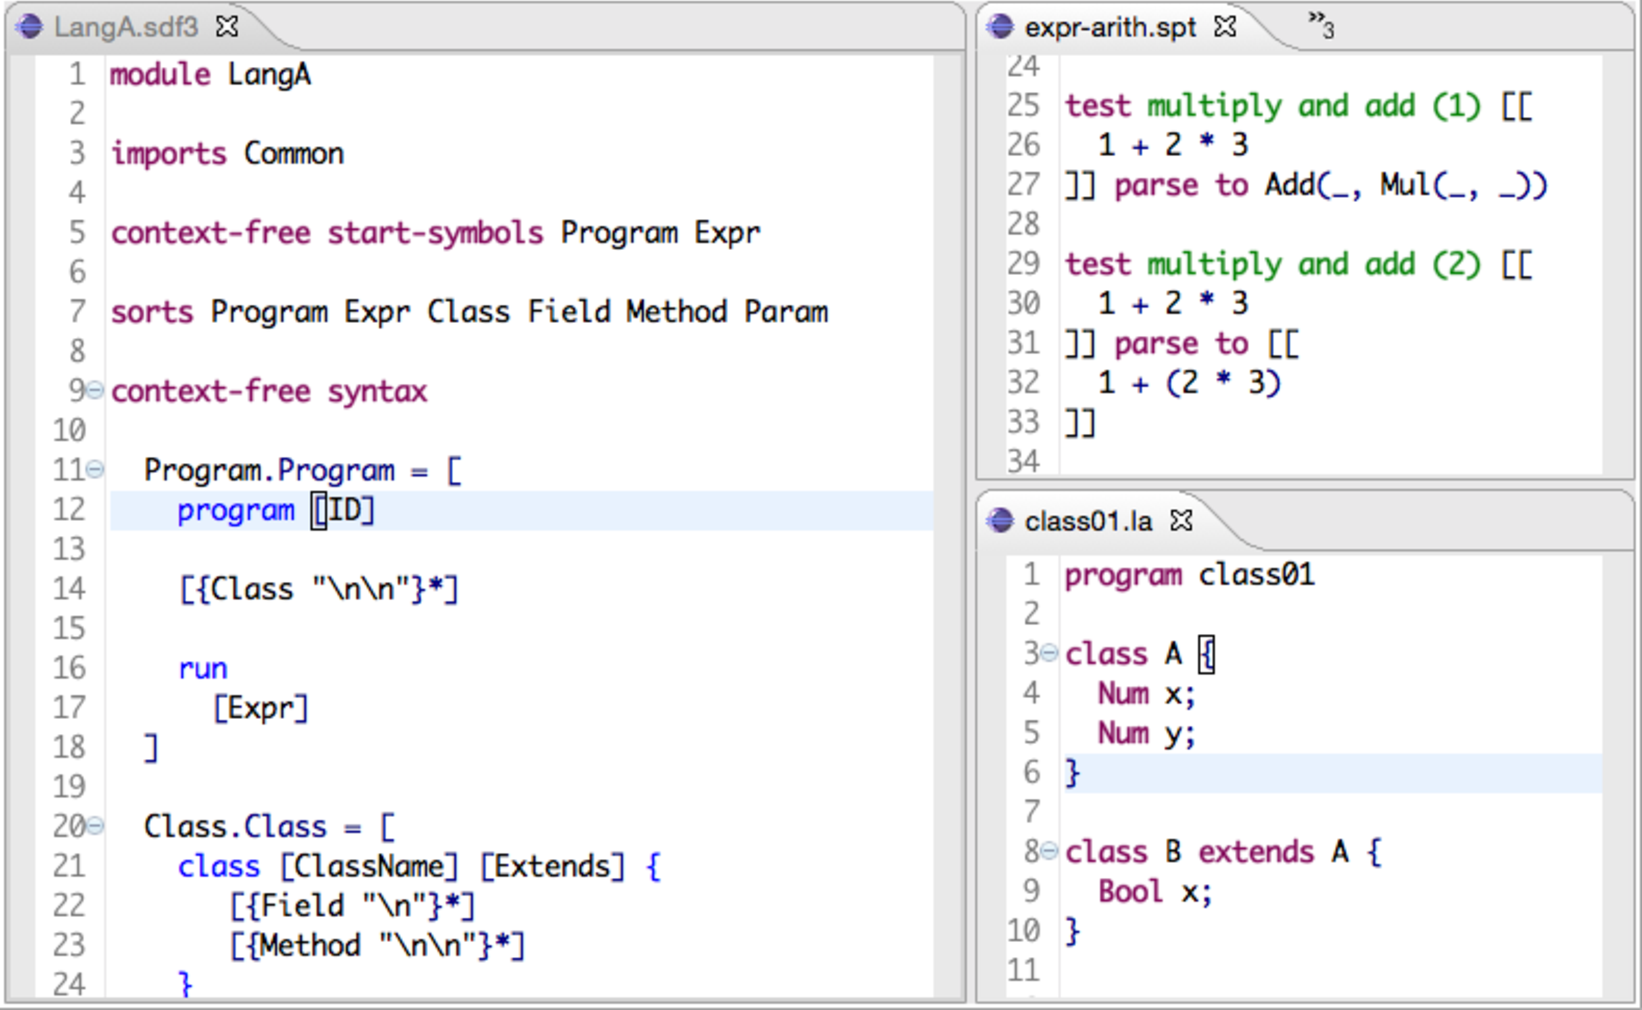
\includegraphics[width=\hsize]{syntax/syntax-dev.pdf}
\caption{Developing and testing syntax definition in the same IDE context.}
\figurelabel{syntax-dev}
\end{figure}


\section{Configuration}

As we indicated in \Chapter{getting-spoofax}, the name that you choose for your
language project is important since it ties a bunch of things in the
configuration of your project together. The main module of the syntax definition
in directory \LanguageFile{LanguageA}{syntax/} has the name of the language.
Thus, we find \LanguageFile{LanguageA}{syntax/LangA.sdf3} in the example
project. Furthermore, the language name is used as prefix of the \texttt{esv}
configuration files in the \LanguageFile{LanguageA}{editor/} directory. The main
configuration module is \LanguageFile{LanguageA}{editor/LangA.main.esv}. It
declares the file extension to be used by programs in the language (\texttt{la})
and the start symbol to be used for such files. By default the start symbol is
set to \texttt{Start}. For \texttt{LanguageA} I have changed it to
\texttt{Program}, since that is the sort in the syntax definition that
represents the content of a file.


\section{Structure of a Syntax Definition}

An SDF3 syntax definition consists of a collection of modules with the following
outline:

\begin{lstlisting}[language=SDF]
module [ModuleName]
imports [ModuleName*]
context-free start-symbols [Symbol*]
[SyntaxSection*]
\end{lstlisting}

A module may import other modules using their declared name. The start symbols
tell the parser with which syntactic sorts to start parsing. While start symbols
may be declared in any module, they are typically declared in the main module of
language. As noted above, when changing the start symbol to something else than
the default \texttt{Start}, this should be changed in the \texttt{main.esv}
module as well.

Let's have a look at the definition of \LanguageRepoRef{LanguageA}. Its main
syntax module defines the sorts \texttt{Program} and \texttt{Expr} as start
symbols and imports the modules \texttt{Programs}, \texttt{Classes}, and
\texttt{Expressions}:

\lstinputlisting[language=SDF]{../languages/LanguageA/syntax/LangA.sdf3}

\section{Concrete and Abstract Syntax}

The programs in \LanguageRepoRef{LanguageA} have a name, then define a list of
zero or more classes, and finally an expression to be executed in the context of
these class definitions. The following is a minimal program in the concrete
syntax of the language that executes the expression \texttt{1} in the context of
no classes:

\lstinputlisting[language=paplj]{../languages/LanguageA/examples/program/program01.la}

Here is the same program in abstract syntax representation:

\lstinputlisting[language=ATerm]{../languages/LanguageA/examples/program/program01.aterm}

The abstract syntax tree is represented as a term with constructors such as
\texttt{Program} and \texttt{Num} creating tree nodes, and strings to represent
lexemes such as identifiers and numbers.

An SDF3 definition defines both the concrete syntax and abstract syntax views of
a language. Here is a (plain version of) the \texttt{Programs} module:

\lstinputlisting[language=SDF]{../languages/LanguageA/syntax/ProgramsPlain.sdf3}

The module imports the syntax of \texttt{Classes} and \texttt{Expressions} and
defines a \emph{context-free syntax production} to define the syntax of
programs. In general, an SDF3 production has the form

\begin{lstlisting}[language=SDF]
  Sort0.C = [lit3 [Sort1] lit2 [Sort2] lit3 ...]
\end{lstlisting}

where \texttt{Sort0} is the non-terminal sort being defined, \texttt{C} is the
abstract syntax tree constructor, and the brackets contain the body of the
production. The body is a sequence of literal symbols, whitespace, and
non-terminal sorts. The notation for productions uses inverted quotation.
Instead of quoting the literal symbols, the sorts are quoted. Thus, a so-called
template production is equivalent to a normal context-free grammar production of
the form:

\begin{lstlisting}[language=SDF]
  Sort0 = "lit3" Sort1 "lit2" Sort2 "lit3"
\end{lstlisting}

Thus, our \texttt{Program} production is equivalent to the context-free grammar
production

\begin{lstlisting}[language=SDF]
  Program = "program" Class* "run" Expr
\end{lstlisting}

defining the concrete syntax notation of programs. By the way, the \texttt{*} in
\texttt{Class*} is the Kleene-star and denotes a sequence of zero or more
strings matching the \texttt{Class} non-terminal sort.

So, what is the use of the constructor? As indicated above, an SDF3 definition
not only defines the concrete syntax (the notation), but also the abstract
syntax, the tree structure representing the underlying structure of the
notation. Thus, for each SDF3 production there is a corresponding algebraic
signature declaration derived by stripping the literals and whitespace from the
production. For the general production form above, we would get the following
constructor declaration:

\begin{lstlisting}[language=Stratego]
  C : Sort1 * Sort2 -> Sort0
\end{lstlisting}

That is, given abstract syntax trees \texttt{t1} and \texttt{t2} of sorts
\texttt{Sort1} and \texttt{Sort2}, respectively, \texttt{C(t1, t2)} is a
well-formed term of sort \texttt{Sort0}.

\Figure{program-sig} shows the Stratego module \texttt{Programs-sig}
with the signature declaration corresponding to our \texttt{Programs} modules.
The constructor declaration for \texttt{Program} describes the structure of the
abstract syntax term that we saw above. Spoofax automatically generates a
signature module in the \texttt{src-gen/signatures} directory of the project for
each SDF3 module.

\begin{figure}[t]
\lstinputlisting[language=Stratego]{../languages/LanguageA/src-gen/signatures/Programs-sig.str}
\caption{Algebraic signature derived from syntax definition module
\texttt{Program}.}
\figurelabel{program-sig}
\end{figure}

\section{Expression Syntax}


\begin{lstlisting}[language=SDF]
module LangA
imports Common
context-free start-symbols Program Expr
context-free syntax
  Exp.Var = ID
  Exp.Mul = [[Exp] * [Exp]]
  Exp.Add = [[Exp] + [Exp]]
\end{lstlisting}

templates \cite{VollebregtKV12}


\section{Disambiguation}

\begin{lstlisting}
module 
context-free syntax
  Exp.Var = ID
  Exp.Mul = [[Exp] * [Exp]] {left}
  Exp.Add = [[Exp] + [Exp]] {left}
context-free priorities
  Exp.Mul > Exp.Add
\end{lstlisting}

\section{Error Recovery}

\cite{JongeKVS12}


\section{Further Reading}

\cite{KatsVW10}: Pure and declarative syntax definition: paradise lost and
regained

\cite{Vis97.thesis}: definition of SDF2

\cite{JongeV11}: An Algorithm for Layout Preservation in Refactoring
Transformations

\cite{BravenboerTV06}: syntax of AspectJ

\cite{KlintV94,BrandSVV02}: disambiguation filters


\cite{BravenboerV08}: Parse table composition
